\subsection{Problems with Runtime Variability}

\begin{frame}<3>{Recap: How to Implement Software Product Lines?}
	\frameImplementSPLs
\end{frame}

\begin{frame}<1>{Recap: Variability and Binding Times}
	\frameVariabilityAndBindingTimes
\end{frame}

\begin{frame}{Recap: Runtime Variability}
	\begin{mycolumns}[t]
		\begin{note}{Basic Principles}
			{\bf Variability with Configuration Options:}
			\begin{itemize}
				\item Conditional statements controlled by configuration options
				\item Global variables vs.\ method parameters
			\end{itemize}
			{\bf Object-Orientation and Design Patterns:}
			\begin{itemize}
				\item Template Method
				\item Abstract Factory
				\item Decorator
			\end{itemize}	
		\end{note}
	\mynextcolumn
		\frameRuntimeVariabilityProblems
	\end{mycolumns}	
\end{frame}

\subsection{Compile-Time Variability}

\begin{frame}{\myframetitle}
	\begin{mycolumns}[widths={50},animation=none]
		\frameRuntimeVariabilityProblems		
	\mynextcolumn
		\uncover<2->{\begin{definition}{Compile-Time Variability\mysource{\fospl\mypage{49}}}
			Compile-time variability is decided before or at compile time. % TODO check quote. mycite?
		\end{definition}}
		\uncover<3->{\begin{note}{}
			{\bf Goals:}
			\begin{itemize}
				\item Only required source code is compiled
				\item Smaller and highly optimized variants
			\end{itemize}				
			{\bf Challenge:}
			\begin{itemize}
				\item How to implement options and alternatives (i.e.,~variability)?
			\end{itemize}	
		\end{note}}
		\uncover<4->{\begin{note}{In this Lecture}
			Simple concepts and techniques for a few variants
		\end{note}}
	\end{mycolumns}	
\end{frame}

\subsection{Ad-Hoc Clone-and-Own}

\begin{frame}{Ad-Hoc Clone-and-Own}
	\begin{mycolumns}[widths={47},animation=none]
		\begin{note}{Clone-and-Own\mysource{\seiwhitepaperspl\mypage{7}}}
			\mycite{Suppose you are developing a new system that seems very similar to one you have built before. You borrow what you can from your previous effort, modify it as necessary, add whatever it takes, and field the product, which then assumes its own maintenance trajectory separate from that of the first product. What you have done is what is called \emph{clone and own}. You certainly have taken economic advantage of previous work; you have reused a part of another system. But now you have two entirely different systems, not two systems built from the same base. This is again \emph{ad hoc reuse}.}
		\end{note}
	\mynextcolumn
		\begin{example}{Cloning Whole Products}
			~\hfill
\includegraphics[width=.2\linewidth]{130}\hfill
\includegraphics[width=.2\linewidth]{230}\hfill~
		\end{example}
		\pause
		\begin{definition}{Clone-and-Own} % TODO source missing
			\begin{itemize}
				\item New variants of a software system are created by copying and adapting an existing variant
				\item Afterwards, cloned variants evolve independently of each other
			\end{itemize}	
		\end{definition}
	\end{mycolumns}	
\end{frame}

% TODO add types of clones
%		\mynote{Types of Software Clones\mysource{\softwareclonedetection\mypage{1167}}}{
%			\begin{itemize}
%			\item Type 1: identical except whitespaces and comments
%			\item Type 2: syntactically similar (e.g., changed identifiers, \ldots)
%			\item Type 3: copied with modifications (e.g., inserted or removed statements)
%			\item Type 4: similar functionality without textual similarities
%			\end{itemize}
%		}

\begin{frame}[fragile]{Example for Ad-Hoc Clone-and-Own}
	\myframeicon{\includegraphics[scale=0.25,page=6]{graphs}}
	\begin{mycolumns}[b,columns=3,widths={43,32},animation=none]
\begin{codetight}{}
class Graph {
	List nodes = new ArrayList();
	List edges = new ArrayList();

	Edge add(Node n, Node m) {
		Edge e = new Edge(n, m);
		e.weight = new Weight();
		nodes.add(n); nodes.add(m); edges.add(e);
		return e;
	}
	Edge add(Node n, Node m, Weight w) {
		Edge e = new Edge(n, m);
		e.weight = w;
		nodes.add(n); nodes.add(m); edges.add(e);
		return e;
	}
	void print() {
		for (int i = 0; i < edges.size(); i++) {
			((Edge) edges.get(i)).print();
		}
	}
}
\end{codetight}
	\mynextcolumn
		\begin{example}{}
			initial graph implementation providing weighted graphs
		\end{example}
\begin{codetight}{}
class Edge {
	Node a, b;
	Weight weight = new Weight();

	Edge(Node a, Node b) {
		this.a = a; this.b = b;
	}
	void print() {
		a.print(); b.print();
		weight.print();
	}
}
\end{codetight}
\begin{codetight}{}
class Weight {
	void print() {...}
}
\end{codetight}
	\mynextcolumn
\begin{codetight}{}
public class Node {
	int id = 0;

	void print() {
		System.out.print(id);
	}
}
\end{codetight}
	\end{mycolumns}
\end{frame}

\begin{frame}[fragile]{Alice's Clone: Unweighted Graphs}
	\myframeicon{
		
\includegraphics[scale=0.25]{alice}%
		\includegraphics[scale=0.25,page=2]{graphs}
	}
	\begin{mycolumns}[b,columns=3,widths={43,32},animation=none]
\begin{codetight}{}
class Graph {
	List nodes = new ArrayList();
	List edges = new ArrayList();

	Edge add(Node n, Node m) {
		Edge e = new Edge(n, m);
		@|e.weight = new Weight();|@
		nodes.add(n); nodes.add(m); edges.add(e);
		return e;
	}
	@|Edge add(Node n, Node m, Weight w) {
		Edge e = new Edge(n, m);
		e.weight = w;
		nodes.add(n); nodes.add(m); edges.add(e);
		return e;
	}|@
	void print() {
		for (int i = 0; i < edges.size(); i++) {
			((Edge) edges.get(i)).print();
		}
	}
}
\end{codetight}
	\mynextcolumn
		\begin{example}{}
			Alice works with unweighted graphs: she copies and adapts the basic implementation
		\end{example}
\begin{codetight}{}
class Edge {
	Node a, b;
	@|Weight weight = new Weight();|@

	Edge(Node a, Node b) {
		this.a = a; this.b = b;
	}
	void print() {
		a.print(); b.print();
		@|weight.print();|@
	}
}
\end{codetight}
\begin{codetight}{}
@|class Weight {
	void print() {...}
}|@
\end{codetight}
	\mynextcolumn
\begin{codetight}{}
public class Node {
	int id = 0;

	void print() {
		System.out.print(id);
	}
}
\end{codetight}
	\end{mycolumns}
\end{frame}

\begin{frame}[fragile]{Alice's Clone: Unweighted Graphs}
	\myframeicon{
		
\includegraphics[scale=0.25]{alice}%
		\includegraphics[scale=0.25,page=2]{graphs}
	}
	\begin{mycolumns}[b,columns=3,widths={43,32},animation=none]
\begin{codetight}{}
class Graph {
	List nodes = new ArrayList();
	List edges = new ArrayList();

	Edge add(Node n, Node m) {
		Edge e = new Edge(n, m);
		nodes.add(n); nodes.add(m); edges.add(e);
		return e;
	}
	void print() {
		for (int i = 0; i < edges.size(); i++) {
			((Edge) edges.get(i)).print();
		}
	}
}
\end{codetight}
	\mynextcolumn
		\begin{example}{}
			Alice works with unweighted graphs: she copies and adapts the basic implementation
		\end{example}
\begin{codetight}{}
class Edge {
	Node a, b;

	Edge(Node a, Node b) {
		this.a = a; this.b = b;
	}
	void print() {
		a.print(); b.print();
	}
}
\end{codetight}
	\mynextcolumn
\begin{codetight}{}
public class Node {
	int id = 0;

	void print() {
		System.out.print(id);
	}
}
\end{codetight}
	\end{mycolumns}
\end{frame}

\begin{frame}[fragile]{Bob's Clone: Colored Graphs}
	\myframeicon{
		
\includegraphics[scale=0.25]{bob}%
		\includegraphics[scale=0.25,page=12]{graphs}
	}
	\begin{mycolumns}[b,columns=3,widths={43,26},animation=none]
\begin{codetight}{}
public class Graph {
	List nodes = new ArrayList();
	List edges = new ArrayList();

	Edge add(Node n, Node m) {
		Edge e = new Edge(n, m);
		nodes.add(n); nodes.add(m); edges.add(e);
		return e;
	}
	void print() {
		for (int i = 0; i < edges.size(); i++) {
			((Edge) edges.get(i)).print();
		}
	}
}
\end{codetight}
	\mynextcolumn
		\begin{example}{}
			Bob works with colored graphs: he is a colleague of Alice and knows her variant, so he copies and adapts Alice's variant
		\end{example}
\begin{codetight}{}
class Edge {
	Node a, b;

	Edge(Node a, Node b) {
		this.a = a; this.b = b;
	}
	void print() {
		a.print(); b.print();
	}
}
\end{codetight}
	\mynextcolumn
\begin{codetight}{}
public class Node {
	int id = 0;
	~Color color = new Color();~

	void print() {
		~Color.setDisplayColor(color);~
		System.out.print(id);
	}
}
\end{codetight}
\begin{codetight}{}
~public class Color {
	static void setDisplayColor(Color c) {...}
}~
\end{codetight}
	\end{mycolumns}
\end{frame}

\subsection{Problems and Discussion}

\begin{frame}{Why is Clone-and-Own Problematic?}
	~\hfill
	\includegraphics[scale=0.25,page=6]{graphs}
	\hfill
	
\includegraphics[scale=0.25]{alice}%
	\includegraphics[scale=0.25,page=2]{graphs}
	\hfill
	
\includegraphics[scale=0.25]{bob}%
	\includegraphics[scale=0.25,page=12]{graphs}
	\hfill~
\end{frame}

\begin{frame}{Clone-and-Own Problems: Feature Combinations}
	\myframeicon{
		
\includegraphics[scale=0.25]{eve}%
		\includegraphics[scale=0.25,page=16]{graphs}
	}
	~

	\begin{mycolumns}[widths={42}]
		\begin{example}{}
			Eve has a new requirement:
			she wants to work with graphs which are both colored and weighted
		\end{example}
	\mynextcolumn
		\begin{note}{}
			\begin{itemize}
				\item Where to start from?
				\item Does Eve know about Bob's and Alice's variants?
				\item If so, how to avoid repeating the work that has been already done by Alice and Bob, respectively?
			\end{itemize}
		\end{note}
	\end{mycolumns}

	~

	\uncover<2->{
		~\hfill
		\includegraphics[scale=0.25,page=6]{graphs}
		\hfill
		
\includegraphics[scale=0.25]{alice}%
		\includegraphics[scale=0.25,page=2]{graphs}
		\hfill
		
\includegraphics[scale=0.25]{bob}%
		\includegraphics[scale=0.25,page=12]{graphs}
		\hfill~
	}
\end{frame}

\begin{frame}[fragile]{Clone-and-Own Problems: Evolution \& Maintenance}
	\myframeicon{
		\includegraphics[scale=0.2,page=6]{graphs}\\[-9mm]
		\includegraphics[scale=0.2,page=26]{graphs}~~~
	}
	\begin{mycolumns}[b,widths={43}]
		\begin{example}{}
			Maintainers of the initial variant refactor the code of the basic implementation
		\end{example}
\begin{codetight}{}
public class Graph {
	...
	Edge add(Node n, Node m) {
		Edge e = new Edge(n, m);
		nodes.add(n); nodes.add(m); edges.add(e);
		e.weight = new Weight();
		return e;
	}
	Edge add(Node n, Node m, Weight w) {
		@|Edge e = new Edge(n, m);|@
		@|nodes.add(n); nodes.add(m); edges.add(e);|@
		?Edge e = add(n, m);?
		e.weight = w;
		return e;
	}
	...
}
\end{codetight} % TODO order of statements not consistent with prior examples: shall we revert the changed order in prior examples?
	\mynextcolumn
		\begin{note}{}
			\begin{itemize}
				\item Who informs Alice, Bob and Eve about the improvement?
				\item How do they know whether the improvement is relevant for them?
				\item If so, how to propagate the improvement to their variant?
			\end{itemize}
		\end{note}

		~

		
\includegraphics[scale=0.15]{alice}%
		\includegraphics[scale=0.15,page=2]{graphs}
		\hfill
		
\includegraphics[scale=0.15]{bob}%
		\includegraphics[scale=0.15,page=12]{graphs}
		\hfill
		
\includegraphics[scale=0.15]{eve}%
		\includegraphics[scale=0.15,page=16]{graphs}
	\end{mycolumns}
\end{frame}

\begin{frame}{Discussion of Clone-and-Own}
	\includegraphics[scale=0.2,page=6]{graphs}
	\hfill
	
\includegraphics[scale=0.2]{alice}%
	\includegraphics[scale=0.2,page=2]{graphs}
	\hfill
	
\includegraphics[scale=0.2]{bob}%
	\includegraphics[scale=0.2,page=12]{graphs}
	\hfill
	
\includegraphics[scale=0.2]{eve}%
	\includegraphics[scale=0.2,page=16]{graphs}
	\hfill
	\includegraphics[scale=0.2,page=26]{graphs}

	\begin{mycolumns}[columns=2,widths={45,55},animation=none]
		\begin{note}{Advantages}
			\begin{itemize}
				\item Simple and straightforward approach
				\item Rapid exploration of new ideas
				\item No upfront investments
			\end{itemize}
		\end{note}
	\mynextcolumn
		\begin{note}{Disadvantages}
			\begin{itemize}
				\item No structured and systematic reuse (copy \& edit)
				\item No flexible combination of features
				\item Maintenance quickly becomes impractical
			\end{itemize}
		\end{note}
	\end{mycolumns}	
	\begin{mycolumns}[columns=3,widths={15,70}]
	\mynextcolumn
		\begin{note}{Towards Managed Clone-and-Own}
			\begin{itemize}
				\item How can we better manage such clone-and-own development?
				\item The traditional answer: Software Configuration Management
				\item In the sequel: Software Configuration Management in practice
			\end{itemize}
		\end{note}
	\mynextcolumn
	\end{mycolumns}
\end{frame}

% TODO add \pic[width=\linewidth,page=24]{lego}
